\chapter{Grundlagen} % DeepL korrigiert

Im folgenden Kapitel sollen konzeptionelle Grundlagen erläutert werden, welche für das Verständnis der Bachelorarbeit notwendig sind.
Im Rahmen dessen erfolgt eine vertiefende Auseinandersetzung mit den Themengebieten Requirements-Engineering und Augmented-Reality.

  \section{Requirements-Engineering}
  Die Bachelorarbeit hat zum Ziel, sogenannte Requirements, also Anforderungen an ein System, zu visualisieren.
  Für das Verständnis der Arbeit ist es daher von entscheidender Bedeutung, sich mit den Grundlagen des Requirements-Engineering vertraut zu machen.

    \titleemph{System}

    Der Begriff \glqq{}System\grqq{} wird gemäß der Definition des International Requirements Engineering Board (IREB) als \glqq{}eine kohärente, abgrenzbare Menge von Elementen, die durch koordiniertes Handeln einen bestimmten Zweck erfüllen\grqq{} definiert \autocite[][]{ireb_cpre_glossary}. 
    Der Begriff \glqq{}System\grqq{} ist also ein Überbegriff für Produkte, Services, Geräte, Prozeduren und Werkzeuge und kann sowohl physisch als auch virtuell sein.
    Ein System kann folglich beispielsweise ein Software-Produkt, ein Fahrzeug oder sogar eine Dienstleistung sein.
    Daher wird auch in dieser Bachelorarbeit das Wort \glqq{}System\grqq{} als Überbegriff für alle Arten von Systemen genutzt.

    \titleemph{Requirements}

    Grundlegend sind Requirements Anforderungen, die an ein System gestellt werden.
    Das IREB definiert sie in ihrem Glossar mit drei Eigenschaften \autocite[][Def. Requirement]{ireb_cpre_glossary}:
    \begin{itemize}
        \item Ein Bedürfnis eines Interesseneigners (Stakeholder)
        \item Eine Eigenschaft oder Fähigkeit, die ein System haben soll
        \item Eine dokumentierte Repräsentation eines Bedürfnisses, einer Fähigkeit oder einer Eigenschaft
    \end{itemize}
  
    Die Aufgabe der Requirements besteht demnach in der Repräsentation und Dokumentation der Bedürfnisse der Stakeholder in Bezug auf das System

    \newpage

    Die Gestaltung von Requirements kann je nach System und sogar je nach Requirement unterschiedlich sein.
    In ihrem Buch \glqq{}Requirements-Engineering und -Management\grqq{} präsentiert Chris Rupp eine Reihe von Beispielen für unterschiedliche Formen von Requirements \autocite[][S. 19]{Rupp2014}:
    \begin{itemize}
        \item User-Stories
        \item Use-Cases
        \item Stories
        \item Formalisierte natürlichsprachliche Requirements
        \item Requirements in Form von Diagrammen (semiformales Modell)
    \end{itemize}

    
    Natürlichsprachliche Requirements können mit geringem Aufwand selbst formuliert werden.
    Allerdings birgt das auch das Risiko von Missverständnissen und Unklarheiten.

    In der Motivation in Kapitel \ref{section:motivation} wurde das Tool reQlab der IT-Designers GmbH angesprochen, in dessen Rahmen diese Bachelorarbeit entstanden ist.
    Das Ziel von reQlab besteht in der Erkennung von Missverständnissen und Unklarheiten in natürlichsprachlichen Requirements, um somit die Qualität der Requirements zu verbessern.
    Daher werden im Umfang dieser Bachelorarbeit nur natürlichsprachliche Requirements genutzt.

    Des Weiteren werden Requirements in funktionale und nicht-funktionale Requirements unterteilt.
    Funktionale Requirements beschreiben \glqq{}die Funktionen, die das System leisten soll, die Informationen die es verarbeiten soll; das gewünschte Verhalten, welches das System an den Tag legen soll\grqq{} \autocite[][S. 12]{Hruschka2023}.

    Der Begriff „nicht-funktionale Requirements“ ist dabei jedoch etwas irreführend, da auch nicht-funktionale Requirements gewissermaßen Funktionen des Systems beschreiben. \newline
    Peter Hruschka beschreibt in seinem Buch „Funktionale Requirements“ mit der Frage: \glqq{}Was soll das System/Produkt tun?\grqq{}
    Nicht-funktionale Requirements hingegen unterteilt er in zwei Kategorien \autocite[][S. 13]{Hruschka2023}:
    \begin{itemize}
      \item Qualitätsanforderungen: \glqq{}Wie gut? Wie schnell? Wie zuverlässig? \ldots\grqq{}
      \item Randbedingungen: \glqq{}Ressourcen, Wiederverwendung, Zukauf, geforderte Technologie \ldots\grqq{}
    \end{itemize}
    
    Diese Unterteilung ist hilfreich zur Strukturierung der Requirements und könnte im User-Interface der Visualisierung genutzt werden, um die Requirements zu kategorisieren.
    
    \titleemph{Stakeholder}

    Der Begriff Stakeholder umfasst laut dem IREB Glossar \glqq{}Personen oder Organisationen, welche die Requirements eines Systems beeinflussen oder die von dem System beeinflusst werden\grqq{} \autocite[][]{ireb_cpre_glossary}.
    Als Stakeholder können beispielsweise die Endnutzer eines Systems bezeichnet werden, die durch das System beeinflusst werden.
    Sie haben ein Bedürfnis an das System, können dieses jedoch nicht selbst umsetzen.
    Im Gegensatz dazu stehen die Auftraggeber bzw. der Produkteigner (Product Owner), welche ebenfalls Stakeholder sind, die aber selbst über die Systementwicklung entscheiden und die Requirements festlegen.

    Eine Vielzahl an Stakeholdern, wie beispielsweise der Product Owner, ist nicht unmittelbar in den täglichen Entwicklungsprozess des Systems involviert und verfügt daher nur über eine begrenzte Übersicht über den aktuellen Stand des Systems.
    Dennoch nehmen sie durch die gestellten Requirements einen maßgeblichen Einfluss auf das System.
    Für eine effiziente Zusammenarbeit zwischen Stakeholdern und Entwicklern ist es unabdinglich, dass die Requirements sowohl den Stakeholdern als auch den Entwicklern klar und verständlich sind.

    Das Verständnis aller Requirements kann insbesondere bei großen und komplexen Systemen herausfordernd sein, da die Zahl der Requirements mit der Komplexität des Systems signifikant ansteigt.
    Die große Menge an Requirements kann in solchen Projekten schnell zu einer gewissen Unübersichtlichkeit führen.
    Daher ist es von entscheidender Bedeutung, die Requirements klar und übersichtlich zu dokumentieren und zu verwalten.

    \titleemph{Requirements-Engineering}

    Requirements-Engineering ist der Prozess, in dem Requirements an ein System erhoben, dokumentiert, analysiert, spezifiziert und validiert werden.
    Laut Chris Rupp besteht Requirements-Engineering dabei aus vier Haupttätigkeiten \autocite[][S.20]{Rupp2014}:
    \begin{itemize}
        \item Wissen vermitteln
        \item Gute Requirements herleiten
        \item Requirements vermitteln
        \item Requirements verwalten
    \end{itemize}
    Requirements-Engineering ist der erste Schritt bei der Entwicklung eines Systems und kann daher große Auswirkungen auf die Qualität und den Erfolg des Systems haben.
    Ein sauberes Requirements-Engineering verhindert Missverständnisse und Unklarheiten und somit Fehler, welche sich durch die Systementwicklung ziehen und dann mit einem hohen finanziellen und zeitlichen Aufwand behoben werden müssen, wenn sie erkannt sind \autocite[][S.20]{Rupp2014}.

    Die vorliegende Bachelorarbeit verfolgt das Ziel, einen innovativen Ansatz zur Vermittlung und Verwaltung von Requirements zu entwickeln, um auf diese Weise die Qualität und Nützlichkeit der Requirements langfristig zu optimieren.
    Des Weiteren soll die Visualisierung der Requirements dazu beitragen, bei umfangreichen Projekten mit einer Vielzahl an Requirements eine bessere Übersicht über diese zu erlangen, um die Verwaltung der Requirements zu erleichtern.
    Die Visualisierung kann den Stakeholdern durch eine verbesserte Übersichtlichkeit möglicherweise helfen, die Requirements besser zu verstehen und so potenzielle Missverständnisse und Unklarheiten zu vermeiden.
    Auf diese Weise können kostspielige Fehler in der Systementwicklung bereits in einem frühen Stadium identifiziert und somit vermieden werden.
    


  \section{Virtual-Reality}
  Die Kenntnis und das Verständnis der Begriffe der Virtual-Reality (VR) sind für das Verständnis von Augmented-Reality von entscheidender Bedeutung.
  Virtual-Reality beschreibt eine Technologie, die es ermöglicht, eine virtuelle Welt zu erschaffen, in der der Nutzer interagieren kann.
  Dafür wird der Nutzer über verschiedenste audiovisuelle Technologien in diese virtuelle Welt versetzt, die durch Computer generiert wird.
  Im Gegensatz zu Augmented-Reality ist die gesamte Umgebung in Virtual-Reality digital. \autocite[vgl.][S.15]{Dalton2023}.

  Der Begriff der Virtual-Reality lässt sich noch genauer in die Begriffe immersive und nicht-immersive Virtual-Reality unterteilen.
  Die folgenden Eigenschaften, die sich auf die Nutzer beziehen, lassen sich als Indikatoren für nicht-immersive Virtual-Reality betrachten:
  \begin{itemize}
    \item Der Nutzer steht nicht im Mittelpunkt.
    \item Der Nutzer ist nicht vollständig von digitalen Inhalten umgeben.
    \item Der Nutzer erfährt die virtuelle Realität als Beobachter anstatt als Teilnehmer.
  \end{itemize}
  Im Gegensatz dazu sind bei immersiver Virtual-Reality alle äußeren Einflüsse so weit wie möglich reduziert und alle Indikatoren sollten auf immersive Virtual-Reality hinweisen.
  Der Nutzer sollte bei immersiver VR das Gefühl haben, sich selbst in der virtuellen Umgebung zu befinden \autocite[vgl.][S.23-24]{Wolfel2023}.
  Daher geht es bei immersiver virtueller Realität oft vor allem um den visuellen Sinn, da dieser am meisten zur Immersion in die virtuelle Welt beiträgt.
  In den meisten immersiven VR-Anwendungen wird jedoch auch der auditive Sinn über Kopfhörer oder Lautsprecher angesprochen, um die Immersion zu steigern.
  Auch der Tastsinn spielt heutzutage eine Rolle, da viele VR-Controller, wie beispielsweise die Meta Quest Touch Plus-Controller, dem Nutzer haptisches Feedback für Interaktionen geben.

  \section{Augmented-Reality}
  Augmented-Reality (AR) ist eine Technologie, die die reale Welt mit digitalen Informationen erweitert.
  Der Ansatz bei AR ist ähnlich wie bei Virtual-Reality, allerdings wird die reale Welt nicht komplett ersetzt, sondern nur erweitert.
  Demnach sieht der Nutzer also weiterhin seine reale Umgebung, diese wird aber durch digitale Informationen ergänzt.

  \newpage

  Auf dem Realitäts-Virtualitäts-Kontinuum von Milgram, welches, wie in Abbildung \ref{fig:rv-continuum} dargestellt, einen fließenden Übergang zwischen Realität und Virtualität beschreibt, liegt Augmented-Reality zwischen der realen Welt und der virtuellen Welt \autocite[vgl.][S.9]{milgram1999}.

  \begin{figure}[H]
    \centering
    
\includegraphics[width=0.9\textwidth]{images/RV-Continuum.png}
    \caption{Realitäts-Virtualitäts-Kontinuum nach Milgram}
    \source{\autocite[][S.9]{milgram1999}}
    \label{fig:rv-continuum}
  \end{figure}

  Daher wird Augmented-Reality dem Überbegriff der Mixed-Reality zugeordnet, da die reale Welt mit der digitalen Welt vermischt wird.
  Infolgedessen ist die Immersion bei Augmented-Reality im Vergleich zu Virtual-Reality oft von geringerer Bedeutung, da die reale Welt stets als Referenzpunkt wahrnehmbar ist.
  Die Intention von AR-Technologien ist nicht die Versetzung des Nutzers in eine andere Welt, sondern die Erweiterung der realen Welt.

  Für diese Erweiterung der Realität müssen die Anzeigegeräte auch Informationen über die echte Umgebung sammeln können.
  Will man beispielsweise dreidimensionale virtuelle Objekte in die reale Welt einfügen, so muss das Anzeigegerät die eigene Position kontinuierlich bestimmen können um die Position und Rotation des virtuellen Objekts anhand der Bewegungen des Nutzers anzupassen.

  Anzeigegeräte für Augmented-Reality haben viele Gemeinsamkeiten mit Anzeigegeräten für Virtual-Reality.
  Die Besonderheit von AR-Anzeigegeräten besteht jedoch darin, dass sie die reale Welt mit digitalen Informationen erweitern.
  Das impliziert, dass die Anzeigegeräte dem Nutzer auch eine Sicht auf die reale Welt ermöglichen und in diese Informationen einblenden müssen.
  Beispielsweise kann das Display eines Anzeigegeräts transparent sein, sodass der Nutzer durch das Display hindurch sehen kann während auf dem Display Daten angezeigt werden können.
  Alternativ kann das Gerät eine oder mehrere Kameras besitzen, dessen Aufnahmen auf undurchsichtige Bildschirme projiziert werden.
  Diese Vorgehensweise wird auch als Image-Passthrough bezeichnet.

  Es gibt verschiedene Arten von Anzeigegeräten, die für die Darstellung von Augmented-Reality genutzt werden können.
  Grundsätzlich lassen sich drei Hauptkategorien unterscheiden: Head-Mounted-Displays, Handheld-Geräte und Spatial-Displays \autocite[][S. 346]{Carmigniani2011}.
  Im Folgenden werden diese drei Kategorien genauer erläutert und anhand von Beispielen veranschaulicht.

  \newpage

  \subsection{Head-Mounted Displays}
    \label{section:hmds}
    Head-Mounted-Displays (HMDs) sind grundsätzlich Bildschirme, die direkt auf dem Kopf des Nutzers getragen werden.
    Ihre Nähe zu den Augen des Nutzers ermöglicht die Abdeckung eines großen Sichtfelds, ohne dass dafür eine große Display-Fläche benötigt wird.
    Folglich sind sie für eine vollständige Immersion im Normalfall kosteneffektiver als großflächige Displays, wie beispielsweise eine Leinwand.
    Allerdings führt die Befestigung am Kopf automatisch zu einer höheren Gewichtsbelastung für den Nutzer, was bei einer längeren Nutzung als unangenehm empfunden werden kann.


    \subsubsection{VR- und AR-Headsets}

    Klassische VR-Headsets kann man sich vorstellen wie eine Skibrille mit zwei Bildschirmen, die auf dem Kopf getragen wird und üblicherweise ein Display hinter jeweils einer Linse pro Auge hat.
    In Abbildung \ref{fig:oculus-quest-3} ist die Meta Quest 3 als Beispiel eines solchen VR- und AR-Headsets dargestellt.
    Durch die zwei Bildschirme -- für welche auch oft ein Bildschirm virtuell in zwei aufgeteilt wird -- wird für jedes Auge ein eigenes, leicht verschobenes Bild erzeugt, wodurch Inhalte in 3D dargestellt werden können.
    Außerdem können sie durch ihre Nähe zu den Augen des Nutzers das volle Sichtfeld des Nutzers abdecken und so eine immersive Erfahrung schaffen.

    \begin{figure}[H]
      \centering
      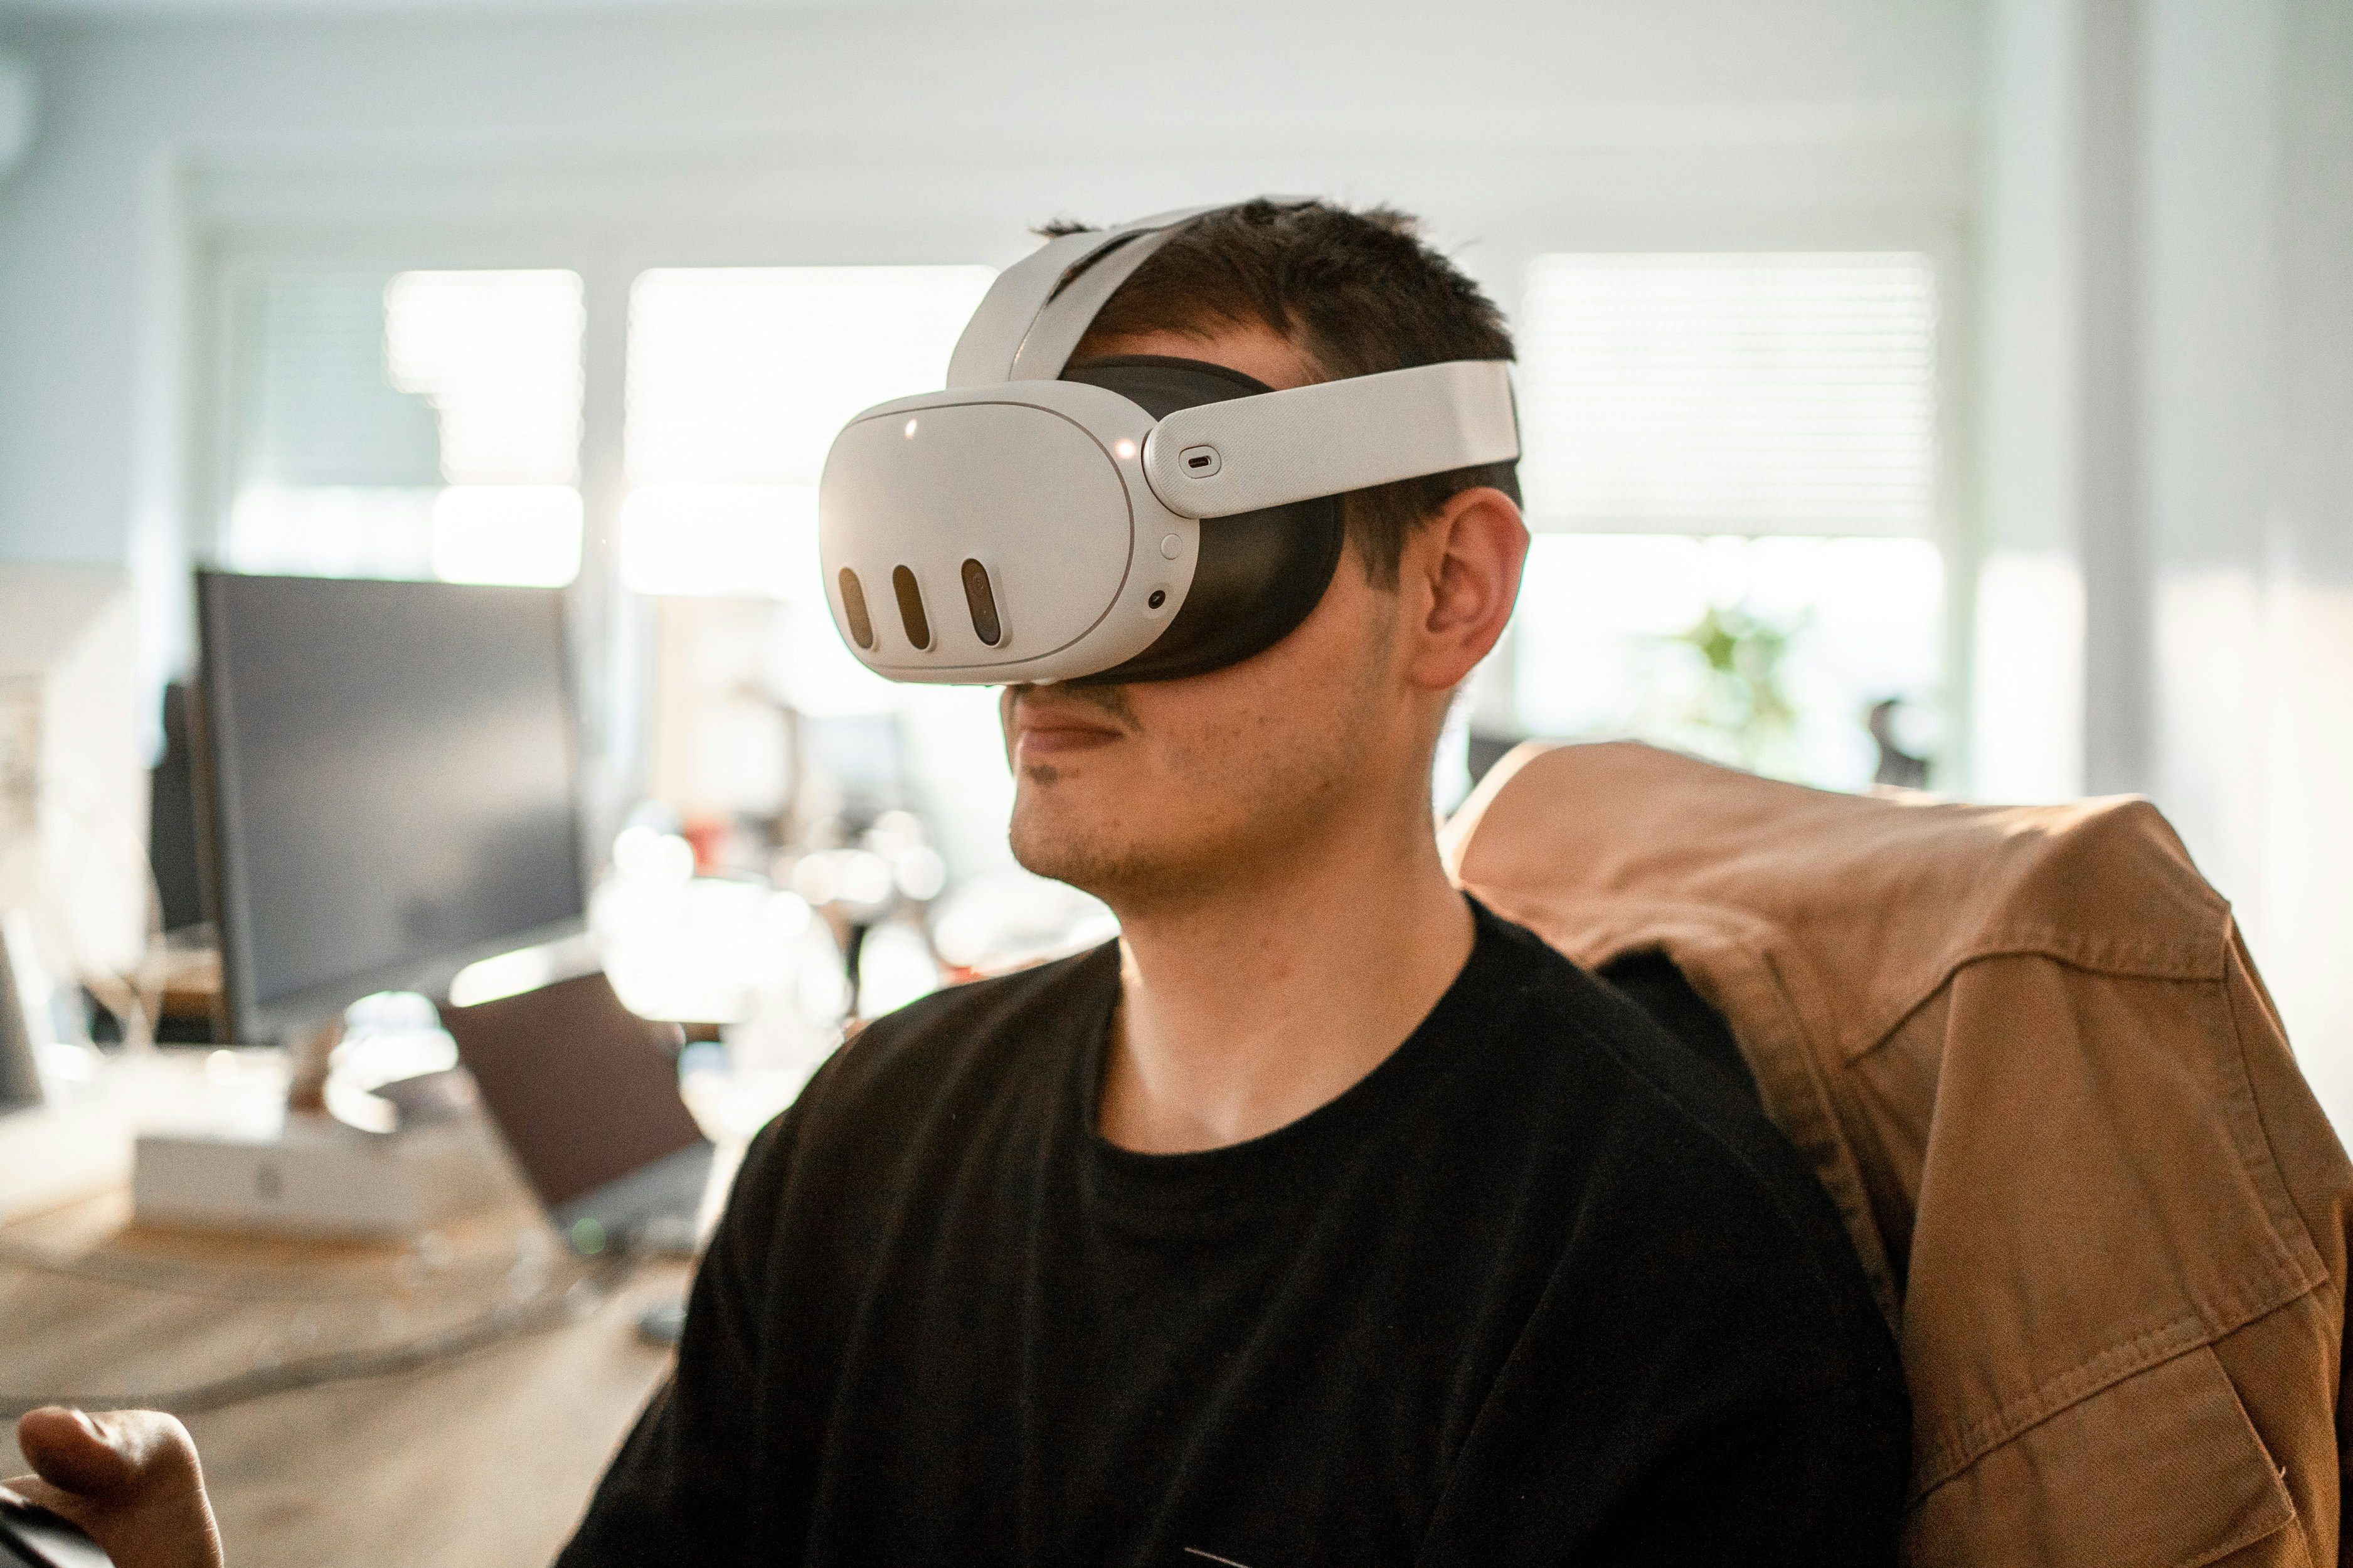
\includegraphics[width=0.9\textwidth]{images/quest3_example.jpg}
      \caption{Meta Quest 3 VR- und AR-Headset}
      \source{\autocite{Quest3Worn}}
      \label{fig:oculus-quest-3}
    \end{figure}

    Die Nähe des Nutzers zu den Displays führt jedoch auch zu visuellen technischen Problemen, wie beispielsweise dem sogenannten Screen-Door-Effekt, bei dem die Zwischenräume zwischen den Pixeln sichtbar sind.
    Die entscheidende Kennzahl in diesem Zusammenhang sind die Pixel per Degree (PPD), welche angibt, wie viele Pixel auf ein Grad des Sichtfelds des Nutzers kommen.
    Eine Möglichkeit um die PPD zu erhöhen und somit den Screen-Door-Effekt zu minimieren, besteht im Einsatz von Displays mit einer hohen Pixeldichte (Pixels per Inch, PPI).
    Beispielsweise hat die Meta Quest 3 eine PPI von 1218 und erreicht damit einen PPD Wert von 25 Pixeln pro Grad \autocite[]{meta-quest-3}.
    Vergleichsweise hat das iPhone 15 Pro eine Pixeldichte von lediglich 460 PPI \autocite[]{iPhone15Pro-datenblatt}.
    Trotz der hohen Pixeldichte des Displays der Meta Quest wirkt das Display des iPhone bei normaler Nutzung aufgrund der Entfernung zum Bildschirm schärfer als das der Meta Quest, auch wenn es eine nicht einmal halb so hohe Pixeldichte aufweist.

    Da die Displays jedoch das gesamte Sichtfeld des Nutzers einnehmen, kann es bei diesen Anzeigegeräten schnell zu Übelkeitsgefühlen kommen, wenn die Bewegungen des Nutzers nicht mit den Bewegungen in der virtuellen Welt übereinstimmen.
    Dem wird so weit wie möglich durch eine hohe Bildwiederholrate der Displays entgegengewirkt, um die Bewegungen des Nutzers möglichst flüssig darzustellen.
    Bei schlecht optimierten Anwendungen kann es jedoch durch Ruckler trotzdem zu Übelkeitsgefühlen kommen.

    Um die Bewegung der Nutzer zu verfolgen und so die virtuelle Welt auf den Bildschirmen anpassen zu können ist eine kontinuierliche Bestimmung der Position des Headsets erforderlich.
    Für diese Bestimmung wird generell zwischen 2 Methoden unterschieden \autocite[]{Gourlay2017}:
    \begin{itemize}
      \item Inside-Out-Tracking: Das Headset trackt seine eigene Position mithilfe von Kameras und Sensoren.
      \item Outside-In-Tracking: Die Position des Headsets wird durch externe Kameras oder Sensoren bestimmt.
    \end{itemize}

    Eine Möglichkeit zur Realisierung von Outside-In-Tracking stellt die Verwendung von Kameras dar, welche im Raum verteilt werden und visuelle Marker am Headset sowie den Steuergeräten tracken.
    Diese Methode ermöglicht eine präzise Positionsbestimmung, allerdings ist der Nutzer durch die festgelegten Trackingstationen in einem bestimmten Raum und den erforderlichen Sichtkontakt zu den Stationen eingeschränkt.
    Des Weiteren ist zu berücksichtigen, dass die Installation der Kameras einen erhöhten Aufwand erfordert, da diese zunächst aufgestellt und kalibriert werden müssen.

    Eine Methode des Inside-Out-Trackings ist das Berechnen der Position durch Daten aus Kameras und 3D-Sensoren im Headset.
    Die Umgebung des Nutzers wird aufgenommen und aus den Kamera- und Sensordaten wird ein 3D-Modell der Umgebung erstellt, um die Position des Headsets zu bestimmen.
    Auf diese Weise wird kontinuierlich eine neue 3D-Repräsentation der Kamera- und Sensordaten erstellt, um die Position des Headsets über die Zeit zu tracken.
    Für diese Methode des Trackings ist jedoch eine hohe interne Rechenleistung notwendig, um die Daten in Echtzeit auf dem Headset selbst verarbeiten zu können.

    Die Interaktion mit der Umgebung erfolgt in der Regel mittels Controllern, deren Position und Rotation ebenfalls kontinuierlich durch Inside-Out- oder Outside-In-Tracking bestimmt werden muss.
    In AR-Headsets mit integrierten Kameras besteht zudem oft die Möglichkeit, die Hände des Nutzers mithilfe der internen Kameras direkt zu tracken und als Eingabegeräte zu nutzen.
    In diesem Zusammenhang können spezifische Gesten oder Handbewegungen als Eingaben identifiziert und zur Interaktion genutzt werden.
    Ein Beispiel für die Interpretation von Gesten ist die Meta Quest 3, welche das Zusammenführen des Zeigefingers und des Daumens als Klick interpretiert.
    Sofern sich die Finger jedoch nicht vollständig berühren, wird dies als Zeigen interpretiert und lässt einen Zeigestrahl an den Fingerspitzen erscheinen.
    
    
    Ursprünglich war die Verbindung eines VR- und AR-Headsets mit einem Computer unabdingbar, um die für die Darstellung der Inhalte erforderliche Rechenleistung zu gewährleisten.
    Im Laufe der Zeit wurden jedoch auch Standalone-VR- und AR-Headsets entwickelt, wie beispielsweise das im Jahr 2024 auf den Markt gebrachte Apple Vision Pro.
    Diese verfügen über eine eigene Rechenleistung, die in der Regel in Form von stromsparenden ARM-Prozessoren realisiert ist, und können somit unabhängig von einem Computer genutzt werden.
    Da sie ohne Kabel auskommen, bieten sie eine größere Bewegungsfreiheit und sind daher besser für Anwendungen geeignet, bei denen sich der Nutzer viel bewegt.

    Allerdings ist nur eine geringe Anzahl von VR-Headsets auch für AR geeignet.
    Die meisten VR-Headsets verfügen über keine Kamera, die für eine qualitativ gute Aufnahme und Wiedergabe der realen Welt geeignet sind.
    Nur Headsets wie beispielsweise die Meta Quest 3, welche in Abbildung \ref{fig:oculus-quest-3} dargestellt ist, oder die Apple Vision Pro besitzen eine oder mehrere hochauflösende Kameras nach außen, um die reale Welt aufzunehmen und so AR durch eine Vermischung aus echter Welt und generierten Daten zu ermöglichen.
    
    Zusammenfassend ermöglicht die neueste Generation von VR- und AR-Headsets durch ihre technische Ausstattung eine besonders hohe Immersion, die durch eine herausragende audiovisuelle Qualität für Anwendungen in AR gekennzeichnet ist.
    Sie sind besonders dafür geeignet, hochauflösende dreidimensionale Inhalte in die reale Welt zu projizieren und so eine immersive Erfahrung zu schaffen.
    Daher werden sie hauptsächlich für Anwendungen eingesetzt, bei denen eine hohe Immersion und eine hohe Qualität der Darstellung von entscheidender Bedeutung sind, wie beispielsweise bei Spielen oder Simulationen.

    Die visuelle Qualität erreicht jedoch noch nicht die Standards moderner Bildschirme für zweidimensionale Betrachtung.
    Während auf modernen Desktop- und Handy-Displays praktisch keine Pixel mehr zu erkennen sind, ist der Pixel-Door-Effekt auch bei den neusten VR- und AR-Headsets noch klar zu sehen.
    Folglich haben sie trotz höheren Pixeldichten eine geringere darstellbare Informationsdichte als klassische zweidimensionale Displays.
    Des Weiteren sind sie für lange Anwendungszeiten und die Verwendung in der Öffentlichkeit in der Regel zu groß und zu schwer, da sie direkt auf dem Gesicht getragen werden müssen.

    Aufgrund der Nähe zu den Augen des Nutzers sind sie mit relativ kleinen Bildschirmen ausgestattet, was sie im Vergleich zu vielen anderen dedizierten Anzeigegeräten für AR und VR zu einer kostengünstigen Alternative macht.
    Die niedrigen Kosten resultieren auch daraus, dass VR-Headsets auch für Videospiele und andere Unterhaltungsanwendungen genutzt werden und daher eine große Nutzerbasis aufweisen.
    So existiert ein weiterer finanzieller Anreiz für die Entwicklung von günstigen VR- und AR-Headsets, da die Hersteller von den hohen Stückzahlen profitieren können.
   

    \subsubsection{Smart-Glasses}

    Smart-Glasses sind Brillen, die digitale Informationen in das Sichtfeld des Nutzers einblenden.
    Sie zeichnen sich durch die Transparenz bzw. Semi-Transparenz der Displays aus, sodass der Nutzer auch ohne Kameras durch die Displays hindurch sehen kann.
    So kann auch ohne digitales Image-Passthrough ein AR-Effekt erzielt werden.
    Des Weiteren ist die Durchsicht durch die Displays meist schärfer als bei Image-Passthrough in VR-Headsets, da direkt die echte reale Welt betrachtet wird und nicht eine imperfekte Kameraaufnahme die auf einem imperfekten Bildschirm wiedergegeben wird.

    Außerdem sind Smart-Glasses meist leichter und kleiner als VR- und AR-Headsets, da sie in der Regel nicht das volle Sichtfeld des Nutzers abdecken müssen und die Technik für Image-Passthrough nicht erforderlich ist.
    Folglich eignen sie sich besser für den Alltag und für längere Anwendungszeiten als konventionelle VR- oder AR-Headsets.
    Zudem verursachen sie durch ihre permanente Transparenz weniger Übelkeitsgefühle bei den Nutzern, da sie sich stets auf die reale Welt als Referenzpunkt beziehen können.

    Aufgrund dieser Eigenschaften werden sie viel als potenzielle Anzeigegeräte für AR in der Arbeitswelt untersucht.
    So haben beispielsweise Forscher der Hochschule Osnabrück und der Universität Osnabrück in nur zwei Logistikunternehmen insgesamt 36 Anwendungsfälle für Smart-Glasses identifiziert \autocite[]{SmartGlasses2017}.


  \subsection{Handheld-Devices}

  Der Begriff \glqq{}Handheld-Device\grqq{} bezeichnet ein Gerät, welches vom Nutzer in der Hand gehalten wird.
  Die Kategorie umfasst heutzutage hauptsächlich Smartphones und Tablets.
  Da die meisten dieser Geräte über eine Kamera und einen Bildschirm verfügen, können sie fast alle für die Darstellung von AR-Inhalten genutzt werden.
  Dazu wird die Kamera sowie diverse Sensoren genutzt, um die Umgebung des Nutzers aufzunehmen und digitale Informationen in das Kamerabild einzublenden.
  Das Smartphone oder Tablet fungiert so als eine Art Fenster in die digitale Welt, durch das der Nutzer die erweiterte Realität wahrnehmen kann.

  Die Immersion ist bei diesem Anzeigegerät jedoch relativ gering, da der Nutzer stets die reale Welt sieht und das Smartphone oder Tablet lediglich ein kleines Fenster in die digitale Welt darstellt.
  Allein durch die Entfernung der Geräte von den Augen der Nutzer können sie nur ein vergleichsweise kleines Sichtfeld abdecken.

  Die Nutzung von Smartphones für AR ist jedoch weit verbreitet, da nahezu jeder ein Smartphone besitzt und somit keine zusätzliche Hardware benötigt wird.
  Beispielsweise hatte das AR-Spiel Pok\'emon Go, welches 2016 veröffentlicht wurde, bereits Anfang 2019 über 1 Milliarde Downloads \autocite[][]{pokemon-go-stats}.
  Bei dem Spiel werden, wie in Darstellung \ref*{fig:pokemon-go} gezeigt ist, sogenannte Pok\'emon über die Smartphone-Kamera in die reale Welt projiziert, sodass der Nutzer sie fangen kann.
  Der Erfolg dieses simplen Konzepts demonstriert das Potenzial der riesigen Nutzergruppe von Smartphones für AR-Anwendungen.


  \begin{figure}[H]
    \centering
    \includegraphics[width=0.9\textwidth]{images/PokemonGo.png}
    \caption{Screenshots aus dem AR-Spiel Pok\'emon Go}
    \label{fig:pokemon-go}
  \end{figure}

  Die genannten Technologien können auch in praktischen Anwendungen zum Einsatz kommen, beispielsweise zur Navigation in Städten oder zur Längenmessung mithilfe von Kameras und Sensoren.

  Des Weiteren besteht die Möglichkeit, Smartphones als Displays für HMDs zu nutzen.
  Allerdings ist in den meisten Fällen die Kamera des Smartphones nicht mehr nutzbar, sodass lediglich die Wiedergabe von VR-Inhalten, jedoch keine AR möglich ist.
  Zudem ist die Pixeldichte von Smartphones meist geringer als bei speziellen VR- und AR-Anzeigegeräten, was die Immersion und Nutzererfahrung verschlechtern kann, da das Display sehr nah an den Augen des Nutzers positioniert ist, wodurch daher starke visuelle Fehler auftreten können.

  \newpage

  \subsection{Spatial-Displays}

  Die bisher vorgestellten Konzepte für AR-Anzeigegeräte basieren auf Displays die direkt am Nutzer selbst befestigt sind.
  Im Gegensatz dazu ist die meiste Technik bei Spatial-Displays in der Umgebung des Nutzers verbaut.
  Der Nutzer selbst muss bei Spatial-Displays meist keine spezielle Hardware tragen, um die AR-Inhalte zu sehen \autocite[]{bimber2006modern}.
  Jedoch können beispielsweise zur Interaktion mit Inhalten Eingabegeräte genutzt werden, die der Nutzer in der Hand hält.

  In den meisten Fällen muss keine spezielle Hardware am Nutzer selbst befestigt werden, was zu einer hohen Immersion durch Spatial-Displays führen kann, wenn die audiovisuelle Immersion auch gegeben ist.
  Auch das ergonomische Nutzererlebnis über lange Zeiträume kann durch Spatial-Displays verbessert werden, da der Nutzer nicht durch das Tragen von schwerer Hardware belastet wird.

  Ein wesentlicher Nachteil von Spatial-Displays ist jedoch der Abstand der Displays zum Nutzer.
  Da sie weiter vom Nutzer entfernt sind als HMDs oder Handheld-Devices können sie mit der gleichen Displaygröße nur ein kleineres Sichtfeld abdecken.
  Daher werden bei Spatial-Displays oft sehr große Displays wie bspw. Beamer genutzt, um trotz der größeren Distanz zum Nutzer ein großes Sichtfeld abzudecken.
  Folglich sind Spatial-Displays mit höheren Kosten und einem größeren Aufwand bei der Installation verbunden als HMDs oder Handheld-Devices.
  Daher werden sie in der Regel in anspruchsvollen Industrieanwendungen eingesetzt und eignen sich meist nicht für den privaten Gebrauch.

  \newpage

  Eine solche industrielle Anwendung ist ein Fahrsimulator von Mercedes -- dargestellt in Abbildung \ref{fig:merc-sim} -- bei der die kompletten Wände von 14 Projektoren bespielt werden, um eine immersive Umgebung für den Fahrsimulator zu schaffen.
  Die Anzeige der Inhalte ist auf die Fahrerposition des Fahrzeugs abgestimmt, sodass der Fahrer das Gefühl hat, sich tatsächlich in einem Fahrzeug zu befinden.
  Mit solchen hoch entwickelten Spatial-Displays können also sehr realistische und immersive Umgebungen geschaffen werden, die für viele Anwendungen, wie bspw. Fahrsimulatoren, sehr nützlich sind.
  Allerdings sind derartige Darstellungsmöglichkeiten mit hohen Kosten und einem erheblichen Aufwand verbunden, der im Vergleich zu anderen Lösungen deutlich höher ist.

  \begin{figure}[H]
    \centering
    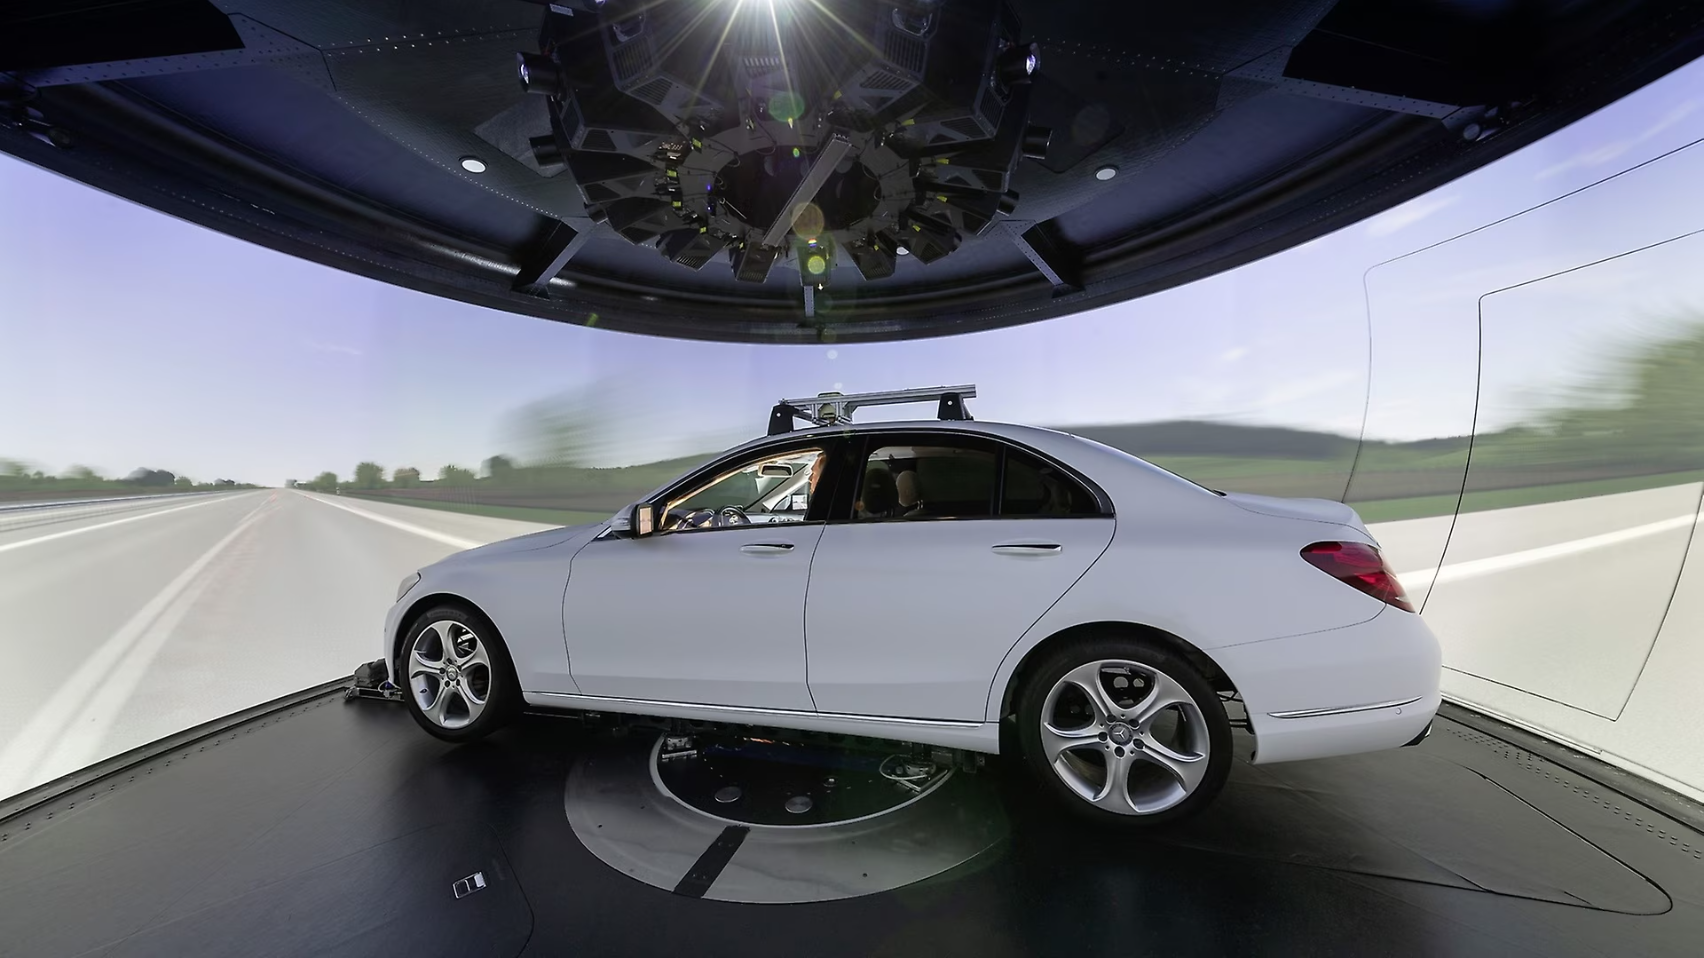
\includegraphics[width=0.8\textwidth]{images/merc-sim.png}
    \caption{Innenraum des Mercedes-Benz Fahrsimulators}
    \source{\autocite{MercedesSimulator}}
    \label{fig:merc-sim}
  \end{figure}

  Betrachtet man Spatial-Displays jedoch nicht nur auf Basis der Immersion, die durch sie erreicht werden kann, ergeben sich auch viele Anwendungsmöglichkeiten für Spatial-Displays, die nicht auf Immersion abzielen.
  Beispielsweise können Spatial-Displays genutzt werden, um Informationen in die reale Welt zu projizieren, die für den Nutzer nützlich sind.
  So zählen auch Head-Up-Displays in Fahrzeugen zu der Kategorie der Spatial-Displays.
  Sie projizieren Informationen in das Sichtfeld des Fahrers, ohne dass sich dieser auf ein Display abseits der Straße vor ihm konzentrieren muss.
  Sie nutzen ähnliche Technologien wie Smart-Glasses, um Informationen auf semi-transparente Displays zu projizieren.

  \newpage
  
\section{Gamification von UX}
\label{sec:gamification-ux}

\glqq{}Gamification ist die Nutzung von Spielmechanismen und -designprinzipien in nicht-spielerischen Kontexten um das Nutzerengagement zu erhöhen\grqq{} \autocite[][S.63]{hillmann2021ux}.
So beschreibt Cornel Hillmann, ein Experte für User-Experience-Design, die Bedeutung von Gamification von UX.

Dieses Prinzip lässt sich aufgrund der hohen Immersion und Interaktivität von VR und AR in XR-Anwendungen besonders gut und quasi standartmäßig nutzen, um das Nutzerengagement zu erhöhen.
Auch durch den Neuheitsfaktor von AR und VR können Nutzer dazu motiviert werden, die Anwendung mehr zu nutzen.

Hillmann gibt drei Hauptbestandteile seines Ansatzes von Gamification von UX an, die in einer Anwendung vorhanden sein müssen, um das Nutzerengagement zu erhöhen \autocite[S.66]{hillmann2021ux}:
\begin{itemize}
  \item Motivation: Die Anwendung muss Elemente enthalten, die den Nutzer zur weiteren Nutzung motivieren.
  \item Herausforderung: Der Nutzer muss eine Herausforderung haben, die er bewältigen kann.
  \item Trigger: Der Nutzer muss für die Herausforderung belohnt werden.
\end{itemize}

Der Ansatz von Hillmann basiert auf der Nutzung der Belohnungsmechanismen von Spielen, um die Motivation der Nutzer zu fördern.
Eine von Hillmann beschriebene Möglichkeit ist die Nutzung von Punkten, um den Fortschritt des Nutzers zu visualisieren und ihn somit zu motivieren, das Arbeiten in der Anwendung fortzusetzen.

Hillmann beschreibt auch, wie Gamification von UX bei der Orientierung, Beruhigung und Onboarding-Problemen der neuen Technologie von XR helfen kann.
So zeigt sich in der Praxis beispielsweise häufig, dass neue Nutzer nicht in die richtige Richtung schauen, um die Inhalte zu sehen, oder von der neuen Technologie überfordert sind.
Daher kann durch eine intelligente Anordnung der Objekte und eine spielähnliche Zielführung die Orientierung sowie die User-Experience der Nutzer verbessert werden \autocite[S.67]{hillmann2021ux}.

% DeepL korrigiert

% 1x Durchgelesen (02.07)